\documentclass[12pt, oneside]{article}
\usepackage[letterpaper, margin=1in]{geometry}
\usepackage[english]{babel}
\usepackage[utf8]{inputenc}
\usepackage{amsmath}
\usepackage{amsfonts}
\usepackage{amssymb}
\usepackage{tikz}
\usepackage{tkz-fct}

\usepackage{fancyhdr}
\pagestyle{fancy}
\fancyhf{}
\rhead{\thepage \\Name: \hspace{1.5in}.\\}
\lhead{BECA / Dr. Huson / 11.2 Algebra 2 \\* 29 May 2018 \\* \textbf{Do Now: Solving by graphing}}

\vspace{1cm}

\renewcommand{\headrulewidth}{0pt}

\title{Problem set template}
\author{Chris Huson}
\date{May 2018}

\begin{document}
%\maketitle

\subsubsection*{\\* \textnormal{Graph carefully using pencil}}

\begin{enumerate}

\item Find algebraically the zeros for $f(x)=x^3-5x^2-4x+20$. (graph is shown) \\[5pt]
%(Based on the graph, find the zeros, then write $f$ in factored form. Then show the work to solve each factor for its zero.)\\*[.5in]
%\begin{left}
    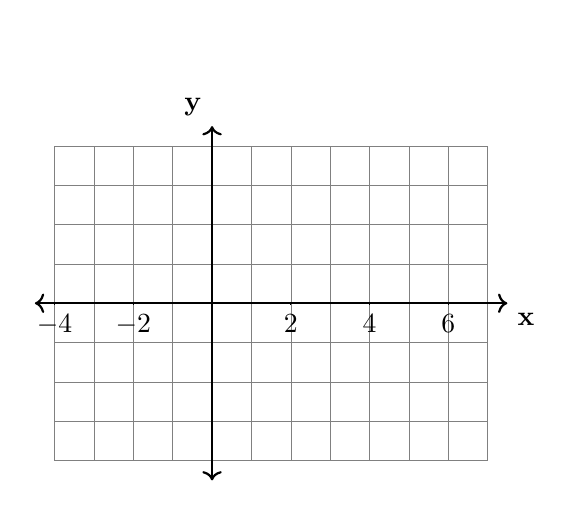
\begin{tikzpicture}[scale=2/4]
    \draw[step=1cm,gray,very thin] (-4,-4) grid (7,4);
    \draw[thick,<->] (-4.5,0) -- (7.5,0) node[anchor=north west] {\textbf{x}};
    \draw[thick,<->] (0,-4.5) -- (0,4.5) node[anchor=south east] {\textbf{y}};
    \foreach \x in {-4, -2, 2, 4, 6} \draw (\x cm,1pt) -- (\x cm,-1pt) node[anchor=north] {$\x$};
    %\foreach \y in {5} \draw (1pt,\y cm) -- (-1pt,\y cm) node[anchor=east] {50}; %{$\y$};
    \tkzInit[xmin=-4,xmax=6,ymin=-4,ymax=7,ystep=1]   
    \tkzFct[color=black,thick,<->,domain = -3:6] {0.1*(x+2)*(x-2)*(x-5)};
    \end{tikzpicture}\\[0.5in]
%\end{left}


\item Find algebraically the zeros for $g(x)=x^3+x^2-6x$. \\*[1.5in]
On the set of axes below, graph $y=g(x)$.
\begin{center}
    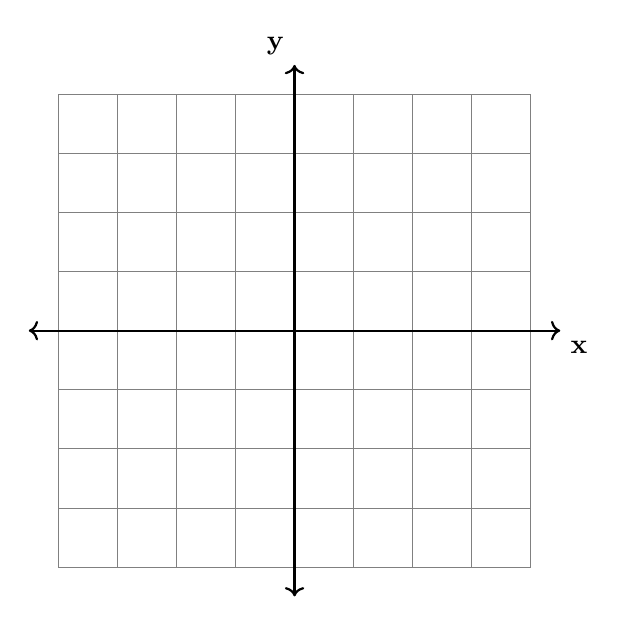
\begin{tikzpicture}[scale=3/4]
    \draw[step=1cm,gray,very thin] (-4,-4) grid (4,4);
    \draw[thick,<->] (-4.5,0) -- (4.5,0) node[anchor=north west] {\textbf{x}};
    \draw[thick,<->] (0,-4.5) -- (0,4.5) node[anchor=south east] {\textbf{y}};
    %\foreach \x in {-4, -2, 2, 4} \draw (\x cm,1pt) -- (\x cm,-1pt) node[anchor=north] {$\x$};
    %\foreach \y in {5} \draw (1pt,\y cm) -- (-1pt,\y cm) node[anchor=east] {50}; %{$\y$};
    %\tkzInit[xmin=-6,xmax=5,ymin=-7,ymax=7,ystep=1]   
    %\tkzFct[color=black,thick,<->,domain = -4.3:4.9] {0.1*(x)*(x+3)*(x-2)};
    \end{tikzpicture}
\end{center}

\newpage

\item Factor completely over the set of integers $f(x)=x^3-3x^2+x-3$. (graph is shown) \\[5pt]
Hint: Get one factor from the graph. Then use long division: divide $f(x) \div (x-?)$.
%(Based on the graph, find the zeros, then write $f$ in factored form. Then show the work to solve each factor for its zero.)\\*[.5in]
%\begin{left}
    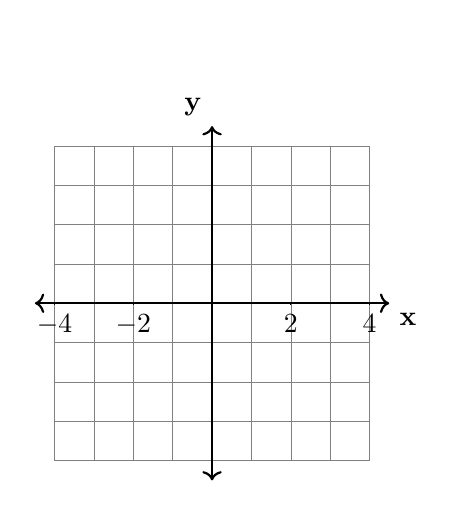
\begin{tikzpicture}[scale=2/4]
    \draw[step=1cm,gray,very thin] (-4,-4) grid (4,4);
    \draw[thick,<->] (-4.5,0) -- (4.5,0) node[anchor=north west] {\textbf{x}};
    \draw[thick,<->] (0,-4.5) -- (0,4.5) node[anchor=south east] {\textbf{y}};
    \foreach \x in {-4, -2, 2, 4} \draw (\x cm,1pt) -- (\x cm,-1pt) node[anchor=north] {$\x$};
    %\foreach \y in {5} \draw (1pt,\y cm) -- (-1pt,\y cm) node[anchor=east] {50}; %{$\y$};
    \tkzInit[xmin=-1.2,xmax=3.7,ymin=-4,ymax=7,ystep=1]   
    \tkzFct[color=black,thick,<->,domain = -.8:3.3] {0.5*(x*x+1)*(x-3)};
    \end{tikzpicture}\\[1in]
%\end{left}


\item Solve the equation $\sqrt{2x+2}+x=3$ algebraically, and justify the solution set.\\*[1in]
 %Alg2 Regents Aug2016
On the set of axes below, graph $y=\sqrt{2x+2}+x$ and $y=3$.\\
Hint: graph it first. $x$ equals the intersection.\\ "Justify" means substitute into the equation.\\*
%\begin{center}
    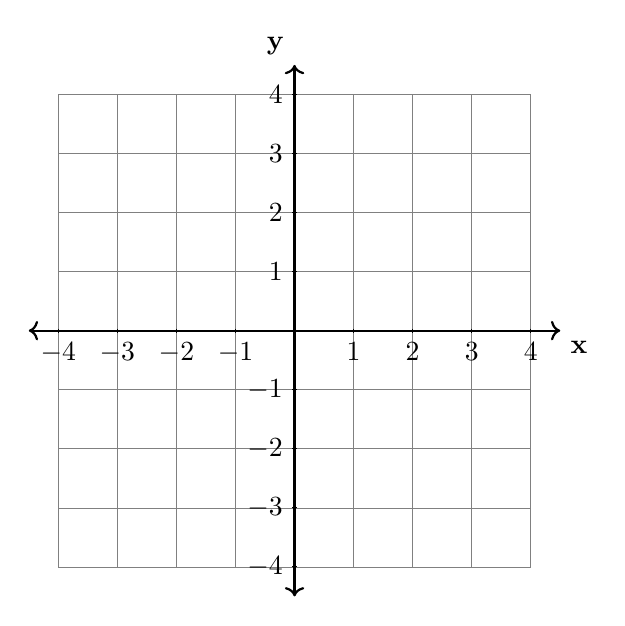
\begin{tikzpicture}[scale=3/4]
    \draw[step=1cm,gray,very thin] (-4,-4) grid (4,4);
    \draw[thick,<->] (-4.5,0) -- (4.5,0) node[anchor=north west] {\textbf{x}};
    \draw[thick,<->] (0,-4.5) -- (0,4.5) node[anchor=south east] {\textbf{y}};
    \foreach \x in {-4,-3, -2,-1,1, 2,3, 4} \draw (\x cm,1pt) -- (\x cm,-1pt) node[anchor=north] {$\x$};
    \foreach \y in {-4,-3, -2,-1,1, 2,3, 4} \draw (1pt,\y cm) -- (-1pt,\y cm) node[anchor=east] {$\y$};
    %\tkzInit[xmin=-6,xmax=5,ymin=-7,ymax=7,ystep=1]   
    %\tkzFct[color=black,thick,<->,domain = -4.3:4.9] {0.1*(x)*(x+3)*(x-2)};
    \end{tikzpicture}
%\end{center}

\newpage

\item Given $N(t)=N_0(e)^{-rt}$, where $N(t)$ is the amount of a drug, $N_0$ is the initial dosage, $r$ is the decay rate, and $t$ is time in hours.\\[5pt] For $A$, model $A(t)$ as an initial amount of 190 milligrams and decay rate of 0.20.\\[5pt]
For $B, B(t)$ is 65 milligrams initially with a decay rate of 0.07.\\*[5pt]
Write equations for $A(t)$ and $B(t)$.\\[.75in]
Graph each function on the set of axes below.
\begin{center}
    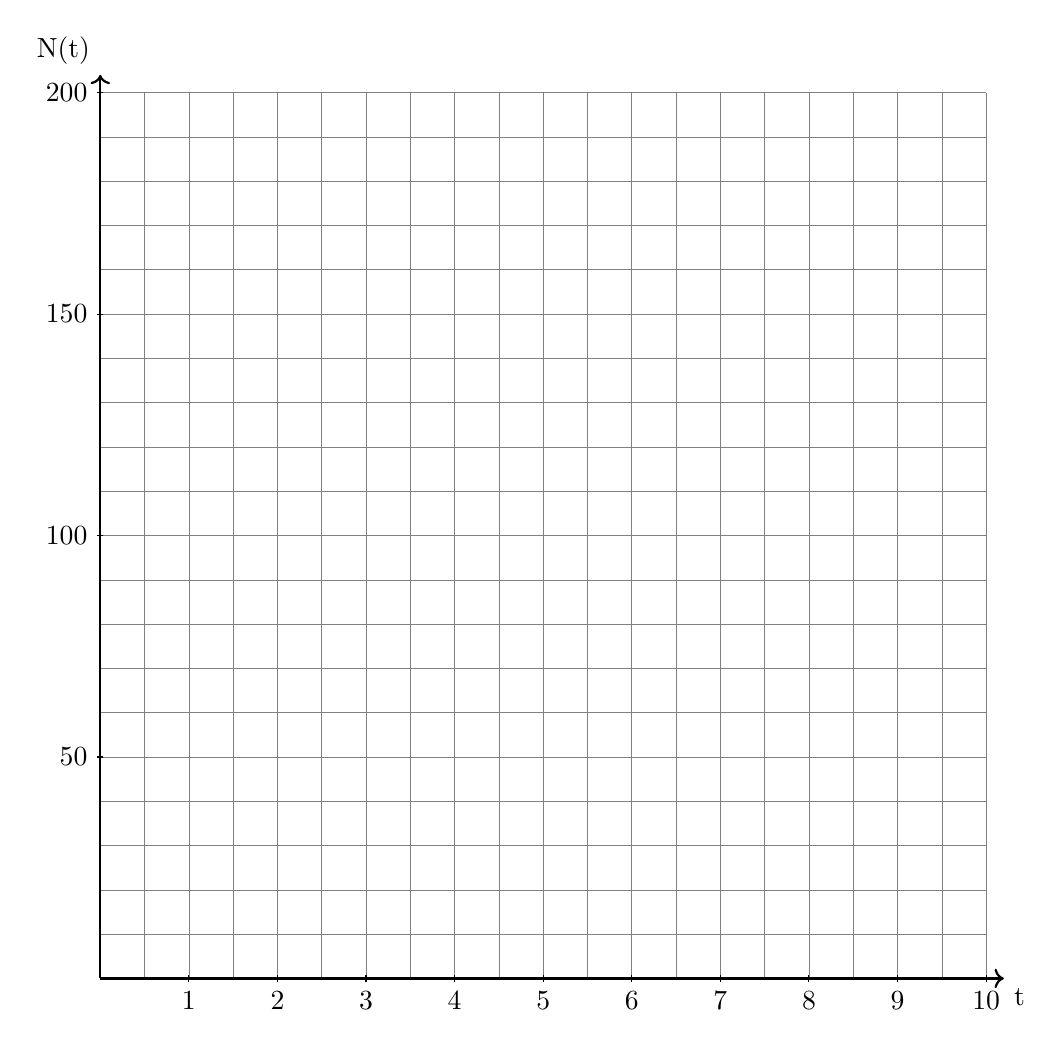
\begin{tikzpicture}[scale=4.5/4]
    \draw[step=0.5cm,gray,very thin] (0,0) grid (10,10);
    \draw[thick,->] (0,0) -- (10.2,0) node[anchor=north west] {t};
    \draw[thick,->] (0,0) -- (0,10.2) node[anchor=south east] {N(t)};
    \foreach \x in {1,2,3,4,5,6,7,8,9,10} \draw (\x cm,1pt) -- (\x cm,-1pt) node[anchor=north] {$\x$};
    \foreach \y in {2.5} \draw (1pt,\y cm) -- (-1pt,\y cm) node[anchor=east] {50};
    \foreach \y in {5} \draw (1pt,\y cm) -- (-1pt,\y cm) node[anchor=east] {100};
    \foreach \y in {7.5} \draw (1pt,\y cm) -- (-1pt,\y cm) node[anchor=east] {150};
    \foreach \y in {10} \draw (1pt,\y cm) -- (-1pt,\y cm) node[anchor=east] {200};
    \end{tikzpicture}
\end{center}
To the \emph{nearest hour}, $t$, when will the two drugs be at equal levels?\\*[0.5in]
When will $145$ milligrams of drug $A$ remain, to the \emph{nearest tenth of an hour}? 

\newpage

\item For each polynomial graph, state 
\begin{enumerate}
\item its degree,
\item how many distinct zeros it has, and
\item the sign of its leading coefficient.
\end{enumerate}

    \begin{tikzpicture}[scale=2/4]
    %\draw[step=1cm,gray,very thin] (-7,-7) grid (7,7);
    \draw[thick,<->] (-7.5,0) -- (7.5,0) node[anchor=north west] {\textbf{x}};
    \draw[thick,<->] (0,-7.5) -- (0,7.5) node[anchor=south east] {\textbf{y}};
    %\foreach \x in {-6, -4, -2, 2, 4, 6} \draw (\x cm,1pt) -- (\x cm,-1pt) node[anchor=north] {$\x$};
    %\foreach \y in {5} \draw (1pt,\y cm) -- (-1pt,\y cm) node[anchor=east] {50}; %{$\y$};
    \tkzInit[xmin=-6,xmax=6,ymin=-7,ymax=7,ystep=1]   
    \tkzFct[color=black,thick,<->,domain = -4.3:5.2] {-0.1*(x+3)*(x)*(x-4)};
    \end{tikzpicture}
    \begin{tikzpicture}[scale=2/4]
    %\draw[step=1cm,gray,very thin] (-7,-7) grid (7,7);
    \draw[thick,<->] (-7.5,0) -- (7.5,0) node[anchor=north west] {\textbf{x}};
    \draw[thick,<->] (0,-7.5) -- (0,7.5) node[anchor=south east] {\textbf{y}};
    %\foreach \x in {-6, -4, -2, 2, 4, 6} \draw (\x cm,1pt) -- (\x cm,-1pt) node[anchor=north] {$\x$};
    %\foreach \y in {5} \draw (1pt,\y cm) -- (-1pt,\y cm) node[anchor=east] {50}; %{$\y$};
    \tkzInit[xmin=-6,xmax=6,ymin=-7,ymax=7,ystep=1]   
    \tkzFct[color=black,thick,<->,domain = -5.3:4.2] {-0.05*(x+5)*(x+3)*(x-1)*(x-4)};
    \end{tikzpicture}
\\[30pt]
    \begin{tikzpicture}[scale=2/4]
    %\draw[step=1cm,gray,very thin] (-7,-7) grid (7,7);
    \draw[thick,<->] (-7.5,0) -- (7.5,0) node[anchor=north west] {\textbf{x}};
    \draw[thick,<->] (0,-7.5) -- (0,7.5) node[anchor=south east] {\textbf{y}};
    %\foreach \x in {-6, -4, -2, 2, 4, 6} \draw (\x cm,1pt) -- (\x cm,-1pt) node[anchor=north] {$\x$};
    %\foreach \y in {5} \draw (1pt,\y cm) -- (-1pt,\y cm) node[anchor=east] {50}; %{$\y$};
    \tkzInit[xmin=-6,xmax=6,ymin=-7,ymax=7,ystep=1]   
    \tkzFct[color=black,thick,<->,domain = -1.3:5.2] {-0.5*(x-2)*(x-2)};
    \end{tikzpicture}
    \begin{tikzpicture}[scale=2/4]
    %\draw[step=1cm,gray,very thin] (-7,-7) grid (7,7);
    \draw[thick,<->] (-7.5,0) -- (7.5,0) node[anchor=north west] {\textbf{x}};
    \draw[thick,<->] (0,-7.5) -- (0,7.5) node[anchor=south east] {\textbf{y}};
    %\foreach \x in {-6, -4, -2, 2, 4, 6} \draw (\x cm,1pt) -- (\x cm,-1pt) node[anchor=north] {$\x$};
    %\foreach \y in {5} \draw (1pt,\y cm) -- (-1pt,\y cm) node[anchor=east] {50}; %{$\y$};
    \tkzInit[xmin=-6,xmax=6,ymin=-7,ymax=7,ystep=1]   
    \tkzFct[color=black,thick,<->,domain = -3.3:5.2] {0.05*(x*x*x*x-3*x*x*x-9*x*x+10*x+20)};
    \end{tikzpicture}


\end{enumerate}
\end{document}
